\title{Лекция 23\\Принципы решения задач в интеллектуальных компьютерных системах нового поколения}
\author[]{Шункевич Д.В.}
\institute[]{Белорусский государственный университет информатики и радиоэлектроники}

\begin{frame}
	\titlepage
\end{frame}

\begin{frame}{\\Содержание лекции}
	\topline
	\justifying
	Стратегии решения задач в компьютерных системах нового поколения. Основные модели логического вывода. Принципы организации логического вывода в интеллектуальных компьютерных системах нового поколения. Принципы реализации параллельной обработки знаний в семантической памяти. Связь с базовым языком программирования для обработки баз знаний. 
\end{frame}

<<<<<<< Updated upstream
\begin{frame}{Стратегии решения задач}
\vspace{20}
=======
\begin{frame}{\\Стратегии решения задач}
\topline
\vspace{30}
 \\
 
>>>>>>> Stashed changes
    В литературе, посвященной построению решателей задач, встречается понятие стратегии решения задач. Определим его как метаметод решения задач, обеспечивающий либо поиск одного релевантного известного метода, либо синтез целенаправленной последовательности акций применения в общем случае различных известных методов. Можно говорить об универсальном метаметоде решения задач, объясняющем всевозможные частные стратегии. В частности, можно говорить о нескольких глобальных стратегиях решения информационных задач в базах знаний.\\
    Пусть в базе знаний появился знак инициированного действия с формулировкой, соответствующей цели, направленной только на изменение состояния базы знаний. И пусть текущее состояние базы знаний не содержит контекст (исходные данные), достаточный для достижения указанной выше цели, т.е. такой контекст, для которого в доступном наборе методов имеется метод, использование которого позволяет достичь указанной выше цели.
\end{frame}

<<<<<<< Updated upstream
\begin{frame}{\large Основные стратегии решения задач}
\vspace{20}
        Для решения задачи, когда исходных данных недостаточно, существует 3 основные подхода:
        \begin{textitemize}
            \item декомпозиция (сведение изначальной цели к иерархической системе и/или подцелей (и/или подзадач) на основе анализа текущего состояния базы знаний и анализа того, чего не хватает в базе знаний для использования ого или иного метода). Формализация понятий действия, задачи, метода, средства, навыка и технологии. При этом наибольшее внимание уделяется методам, для создания условий использования которых требуется меньше усилий. В конечном счете мы должны дойти (на самом нижнем уровне иерархии) до подцелей, контекст которых достаточен для применения одного из имеющихся методов (программ) решения задач;
            \item генерация новых знаний в семантической окрестности формулировки изначальной цели с помощью любых доступных методов в надежде получить такое состояние базы знаний, которое будет содержать нужный контекст (достаточные исходные данные) для достижения изначальной цели с помощью какого-либо имеющегося метода решения задач;
=======
\begin{frame}{\\Основные стратегии решения задач}
\topline
\vspace{40}
 \\
 
        Для решения задачи, когда исходных данных недостаточно, существует 3 основные подхода:
        \begin{textitemize}
            \item декомпозиция (сведение изначальной цели к иерархической системе подцелей и/или подзадач путём анализа текущего состояния базы знаний и того, чего не хватает для использования того или иного метода). При этом наибольшее внимание уделяется методам, для использования которых требуется выполнить меньше действий. В конечном счете мы должны дойти до подцелей, контекст которых достаточен для применения одного из имеющихся методов решения задач;
            \item генерация новых знаний в семантической окрестности формулировки изначальной цели с помощью любых доступных методов для получения такого состояния базы знаний, которое будет содержать нужный контекст (достаточные исходные данные) для достижения изначальной цели с помощью какого-либо имеющегося метода решения задач;
>>>>>>> Stashed changes
            \item комбинация первого и второго подходов.
        \end{textitemize}
\end{frame}

\begin{frame}{\\Задачи логики}
<<<<<<< Updated upstream
        Логика решает задачи доказательства истинности высказываний, аргументации того или иного высказывания, задачу генерации и опровержения гипотез. Некоторые гипотезы могут быть опровергнуты, однако извлекая причины того, почему гипотеза опровергнута, можно изменить посылку гипотезы так, чтобы создать новую гипотезу, которая впоследствии может стать теоремой.
\end{frame}

\begin{frame}{\\Логический вывод}
    \vspace{10mm}
=======
\topline
\vspace{30}
 \\
 
        Логика решает задачи доказательства истинности высказываний, аргументации того или иного высказывания, задачу генерации и опровержения гипотез. Некоторые гипотезы могут быть опровергнуты, однако извлекая причины того, почему гипотеза опровергнута, можно изменить посылку гипотезы так, чтобы создать новую гипотезу, которая впоследствии может стать теоремой.
        Современная логика изучает \textit{формальные языки}, служащие для выражения логических рассуждений. \textit{логический язык} — \textit{формальный язык}, предназначенный для воспроизведения логических форм контекстов \textit{естественного языка}, а также выражения логических законов и способов правильных рассуждений в логических теориях, строящихся в данном языке. Логика не изучает то, как были получены знания, она позволяет представлять знания, а также из существующих знаний вывести новые (то есть из имеющихся формул логики вывести новые формулы этой же логики), установить правильность рассуждений.
\end{frame}

\begin{frame}{\\Логический вывод}
\topline
\vspace{40}
 \\
 
>>>>>>> Stashed changes
        Предметная область логических формул, высказываний и формальных теорий задаёт денотационную семантику логических формул, высказываний и формальных теорий и содержит формальную спецификацию понятий, необходимых для формирования логических формул и высказываний любых логик, в том числе традиционных, нечётких, правдоподобных, темпоральных, логик умолчания и любых других. Логические формулы и высказывания интерпретируются с помощью понятий, описанных в Предметной области логических моделей решения задач, включающую модель и реализацию абстрактных агентов, необходимых для решения логических задач. Эта предметная область включает в себя спецификацию таких понятий, как логический вывод, правила вывода, равносильные преобразования и аксиомные схемы.
\end{frame}

\begin{frame}{\\Формальные языки}
<<<<<<< Updated upstream
=======
\topline
>>>>>>> Stashed changes
        Современная логика изучает формальные языки, служащие для выражения логических рассуждений. Логический язык — формальный язык, предназначенный для воспроизведения логических форм контекстов естественного языка, а также выражения логических законов и способов правильных рассуждений в логических теориях, строящихся в данном языке.
        \\Язык SCL — подъязык SC-кода для записи логических утверждений. Над высказываниями языка SCL можно проводить логический вывод.
\end{frame}

\begin{frame}{\\Вывод в формальной системе}
<<<<<<< Updated upstream
    \vspace{10mm}
        Выводом в формальной системе называется любая последовательность формул, где любая формула либо аксиома этой формальной системы, либо непосредственное следствие каких-либо предыдущих формул по одному из правил вывода. Идея выводимости центральна в логике: в любой формальной аксиоматической теории ‘теорема’ – это формула, которая выводится из аксиом. Правильность умозаключений вводится и проверяется совершенно формально, без какой-либо связи с истинностью входящих в него посылок, т.е. исключительно с точки зрения структуры рассуждения. Если нам удалось доказать, пользуясь методами формальной логики, правильность рассуждения, и нам известно из опыта, что все используемые посылки истинны, то мы можем быть уверены в истинности заключения. Истинность используемых посылок задаётся состоянием базы знаний.
\end{frame}

\begin{frame}{\\Логические методы решения задач}
    \vspace{10mm}
    \begin{textitemize}
        \item Классический дедуктивный вывод. Наиболее популярный метод при построении автоматических решателей задач, так как всегда дает достоверный результат. Дедуктивный вывод включает в себя прямой и обратный логический вывод (принцип резолюции, процедуру Эрбрана и др.), все виды силлогизмов и т.д. Основной проблемой дедуктивного вывода является невозможность его использования в ряде случаев, когда отсутствуют достоверные знания. (Sethy S.S.MediaIS-2021art, Averin A.I..UsingPiDI-2004art)
        \item Индуктивный вывод. Предоставляет возможность в процессе решения использовать различные предположения, что делает его удобным для использования в слабоформализованных и трудноформализуемых предметных областях, например при построении систем медицинской диагностики. (Norton J.D..aDemonstrationotIoCoII-2019art, YuxuanZ..MissiEAKGIItDGLaT-2022art)
=======
\topline
    \vspace{10}
     \\
     
        Выводом в формальной системе называется любая последовательность формул такая, что любая формула либо аксиома этой формальной системы, либо непосредственное следствие каких-либо предыдущих формул по одному из правил вывода. Идея выводимости центральна в логике: в любой формальной аксиоматической теории ‘теорема’ – это формула, которая выводится из аксиом. Правильность умозаключений вводится и проверяется совершенно формально, без какой-либо связи с истинностью входящих в него посылок, т.е. исключительно с точки зрения структуры рассуждения. Если нам удалось доказать, пользуясь методами формальной логики, правильность рассуждения, и нам известно из опыта, что все используемые посылки истинны, то мы можем быть уверены в истинности заключения. Истинность используемых посылок задаётся состоянием базы знаний.
\end{frame}

\begin{frame}{\\Логические методы решения задач}
\topline
    \vspace{10}
     \\
     
    \begin{textitemize}
        \item Классический дедуктивный вывод. Наиболее популярный метод при построении автоматических решателей задач, так как всегда дает достоверный результат. Дедуктивный вывод включает в себя прямой и обратный логический вывод (принцип резолюции, процедуру Эрбрана и др.), все виды силлогизмов и т.д. Основной проблемой дедуктивного вывода является невозможность его использования в ряде случаев, когда отсутствуют достоверные знания.
        \item Индуктивный вывод. Предоставляет возможность в процессе решения использовать различные предположения, что делает его удобным для использования в слабоформализованных и трудноформализуемых предметных областях, например при построении систем медицинской диагностики.
>>>>>>> Stashed changes
    \end{textitemize}
\end{frame}
\begin{frame}{}
    \begin{textitemize}
<<<<<<< Updated upstream
        \item  Абдуктивный вывод. Под абдуктивным выводом в искусственном интеллекте, как правило, понимается вывод наилучшего абдуктивного объяснения, т.е. объяснения некоторого события, ставшего неожиданным для системы. Причем наилучшим считается такое объяснение, которое удовлетворяет специальным критериям, определяемым в зависимости от решаемой задачи и используемой формализации. (Safawi A.R..tDecisPoAI-2015art, Gungov A.tAmpliLiDtAoAIiCR-2018art)
        \item Нечеткая логика. Теория нечетких множеств и, соответственно, нечетких логик, также применяется в системах, связанных с трудноформализуемыми предметными областями. Здесь импликативные высказывания могут рассматриваться как "если истинна посылка, то с некоторой вероятностью (часто или редко) истинно заключение", в отличие от классической логики, где зачастую используются статические предметные области и выражение "часто или редко" не применимо. (Uehara K..FuzzyIIPaP-2017art, Geramian A..FuzzyISAfFAiAI-2017art, Son L.H..PictuISaNFISoPFS-2017art)
=======
        \item  Абдуктивный вывод. Под абдуктивным выводом в искусственном интеллекте, как правило, понимается вывод наилучшего абдуктивного объяснения, т.е. объяснения некоторого события, ставшего неожиданным для системы. Причем наилучшим считается такое объяснение, которое удовлетворяет специальным критериям, определяемым в зависимости от решаемой задачи и используемой формализации.
        \item Нечеткая логика. Теория нечетких множеств и, соответственно, нечетких логик, также применяется в системах, связанных с трудноформализуемыми предметными областями. Здесь импликативные высказывания могут рассматриваться как "если истинна посылка, то с некоторой вероятностью (часто или редко) истинно заключение", в отличие от классической логики, где зачастую используются статические предметные области и выражение "часто или редко" не применимо. 
>>>>>>> Stashed changes
    \end{textitemize}
\end{frame}
\begin{frame}{}
    \begin{textitemize}
<<<<<<< Updated upstream
        \item Логика умолчаний. Логика умолчаний применяется, в том числе, для того, чтобы оптимизировать процесс рассуждений, дополняя процесс достоверного вывода вероятностными предположениями в тех случаях, когда вероятность ошибки крайне мала. (Lupea M.aTheorPfCaRDL2002art, Weydert E.DefauLaPaTP-2022art)
        \item Темпоральная логика. Её применение является очень актуальным для нестатичных предметных областей, в которых истинность того или иного утверждения меняется со временем, что существенно влияет на ход решения какой-либо задачи. (Chen G..TempoLIfFDoSSwGPD-2021art, Рыбаков В.В.МультВНЛЛПД-2020ст)        
=======
        \item Логика умолчаний. Логика умолчаний применяется, в том числе, для того, чтобы оптимизировать процесс рассуждений, дополняя процесс достоверного вывода вероятностными предположениями в тех случаях, когда вероятность ошибки крайне мала. 
        \item Темпоральная логика. Её применение является очень актуальным для нестатичных предметных областей, в которых истинность того или иного утверждения меняется со временем, что существенно влияет на ход решения какой-либо задачи.      
>>>>>>> Stashed changes
    \end{textitemize}  
\end{frame}


\begin{frame}{\large Принципы организации логического вывода в интеллектуальных компьютерных системах нового поколения}
<<<<<<< Updated upstream
    \vspace{15mm}
        Технология OSTIS позволяет интегрировать любые модели решения задач и принципы логического вывода для решения задач в интеллектуальных системах на основе общей формальной модели. Для того, чтобы использовать какую-либо новую или существующую модель, необходимо привести ее к предлагаемому формализму, что позволит интегрировать и синхронизировать ее с уже имеющимися в соответствующей библиотеке совместимых компонентов. Формализм SC-кода позволяет описывать отношения между понятиями любой формы и сложности, что делает его подходящим вариантом для использования логического вывода в интеллектуальных компьютерных системах нового поколения. А также воспользоваться техникой иерархии за счёт онтологического подхода, лежащего в основе баз знаний ostis-систем.
        Наследование предметных областей позволяет использовать описанные логики и их компоненты при описании любых логик. Базовые понятия позволяют разработчикам интеллектуальной системы добавлять новые логики. Для реализации конкретной логической модели решения задач необходимо создать предметную область, которая будет дочерней по отношению к Предметной области логических моделей решения задач и предметной области некоторого логического языка, например, языка логики высказываний, языка логики предикатов, языка нечёткой логики и других.
\end{frame}

\begin{frame}{\\Абстрактный SC-агент}
\vspace{12mm}
Абстрактная scl-машина является машиной логического вывода и относится к классу абстрактных sc-машин. Внутренним языком scl-машины является графовый логический язык SCL, её операции соответствуют правилам логического вывода. Семейство специализированных абстрактных графодинамических машин обработки знаний является формальным уточнением операционной семантики указанных выше специализированных графовых языков представления знаний, каждому из которых соответствует одна или несколько абстрактных машин. Эти абстрактные машины соответствуют различным моделям решения задач, логикам, моделям правдоподобных рассуждений. Агент из семейства агентов логического вывода может представлять собой какое-либо правило вывода, применяемое для решения логической задачи. Кроме того, необходимы агенты для выполнения равносильных преобразований логической формулы (например, записать формулу эквиваленции как конъюнкцию двух дизъюнкций) и другие агенты, помогающие применять правила вывода на множестве формул языка логики.
\end{frame}

\begin{frame}{\\Виды абстрактных SC-Агентов}  
    \scnheader{Абстрактная scl-машина}
		\begin{scnrelfromset}{декомпозиция абстрактного sc-агента*}
			\scnitem{Абстрактный sc-агент применения правила вывода}
            \scnitem{Абстрактный sc-агент эквивалентных преобразований логической формулы}
            \scnitem{Абстрактный sc-агент прямого логического вывода}
			\scnitem{Абстрактный sc-агент обратного логического вывода}
		\end{scnrelfromset}	
\end{frame}

\begin{frame}{\Large Абстрактный sc-агент применения правила вывода}
\vspace{8mm}
=======
    \topline
    \vspace{30}
     \\
     
        Технология OSTIS позволяет интегрировать любые модели решения задач и принципы логического вывода для решения задач на основе общей формальной модели. Чтобы использовать какую-либо новую или существующую модель, нужно привести ее к предлагаемому формализму, что позволит интегрировать и синхронизировать ее с уже имеющимися в соответствующей библиотеке компонентов. Формализм SC-кода позволяет описывать отношения между понятиями любой формы и сложности, что делает его подходящим вариантом для использования логического вывода в интеллектуальных компьютерных системах нового поколения.
        Наследование предметных областей позволяет использовать описанные логики и их компоненты при описании любых логик. Базовые понятия позволяют разработчикам интеллектуальной системы добавлять новые логики. Для реализации конкретной логической модели решения задач необходимо создать предметную область, которая будет дочерней по отношению к Предметной области логических моделей решения задач и предметной области некоторого логического языка, например, языка логики высказываний, языка логики предикатов, языка нечёткой логики и других.
\end{frame}

\begin{frame}{\\Абстрактная SCL-машина}
\topline
\vspace{12mm}
 \\
 
Абстрактная scl-машина является машиной логического вывода и относится к классу абстрактных sc-машин. Внутренним языком scl-машины является графовый логический язык SCL, её операции соответствуют правилам логического вывода. Семейство специализированных абстрактных графодинамических машин обработки знаний является формальным уточнением операционной семантики указанных выше специализированных графовых языков представления знаний, каждому из которых соответствует одна или несколько абстрактных машин. Эти абстрактные машины соответствуют различным моделям решения задач, логикам, моделям правдоподобных рассуждений. Агент из семейства агентов логического вывода может представлять собой какое-либо правило вывода, применяемое для решения логической задачи. Кроме того, необходимы агенты для выполнения равносильных преобразований логической формулы (например, записать формулу эквиваленции как конъюнкцию двух дизъюнкций) и другие агенты, помогающие применять правила вывода на множестве формул языка логики.
\end{frame}

\begin{frame}{\\Виды абстрактных SC-Агентов} 
\topline
    \begin{SCn}
\scnheader{Абстрактная scl-машина}
\begin{scnrelfromset}{декомпозиция абстрактного sc-агента}
	\scnitem{Абстрактный sc-агент применения правила вывода}
	\scnitem{Абстрактный sc-агент эквивалентных преобразований логической формулы}
	\scnitem{Абстрактный sc-агент прямого логического вывода}
	\scnitem{Абстрактный sc-агент обратного логического вывода}
\end{scnrelfromset}
\scnhaselement{Реализации интерпретатора логических моделей решения задач}
\begin{scnindent}
	\scnidtf{Реализация scl-машины}
	\scntext{адрес компонента}{https://github.com/ostis-ai/scl-machine}
\end{scnindent}
\end{SCn}
\end{frame}

\begin{frame}{Абстрактный sc-агент применения правила вывода}
\topline
\vspace{8mm}
 \\

>>>>>>> Stashed changes
  Абстрактный sc-агент применения правила вывода применяет заданное правило вывода с заданными логическими формулами. Агент активируется при появлении в sc-памяти инициированного действия, принадлежащего классу действие применение правила вывода. После проверки sc-агентом условия инициирования выполняется процесс применения правила вывода, который заключается в проверке, существует ли в sc-памяти структуры, соответствующие условию применения данного правила и генерации sc-конструкций в соответствии с применяемым правилом. Агент применения правила вывода зачастую используется в процессе работы агентов прямого логического вывода, обратного логического вывода и других агентов.  
\end{frame}

\begin{frame}{}
\begin{figure}[H]
	\caption{SCg-текст. Формализация правила вывода Modus ponens}
	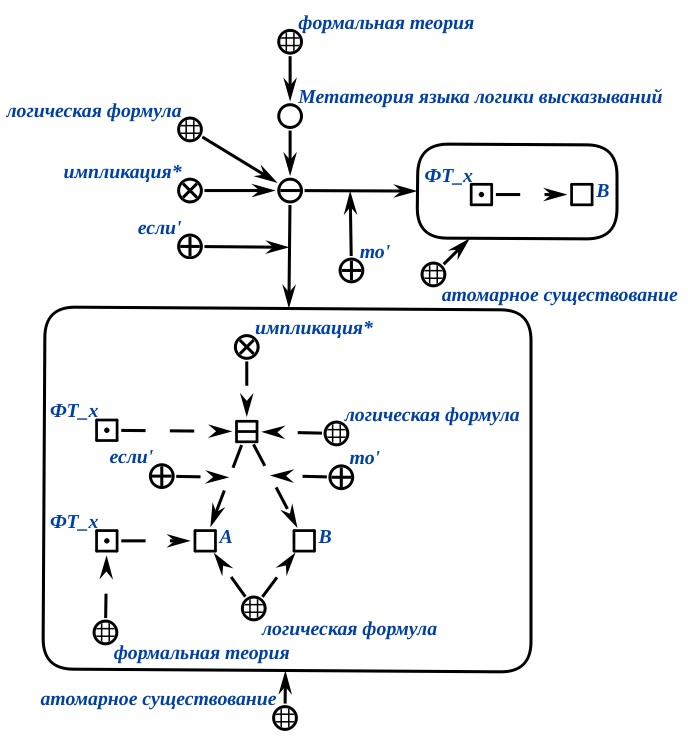
\includegraphics[width=0.9\linewidth, height=8cm]{figures/sc-agents/Modus_ponens.png}
\end{figure}
\end{frame}

\begin{frame}{\Large Абстрактный sc-агент эквивалентных преобразований логической формулы}
<<<<<<< Updated upstream
\vspace{10mm}
  Абстрактный sc-агент эквивалентных преобразований логической формулы применяет некоторые правила, которые приводят логическую формулу в определённый вид. Агент активируется при появлении в sc-памяти инициированного действия, принадлежащего соответствующему классу действий. После проверки sc-агентом условия инициирования выполняется процесс преобразования формулы из одной формы в другую, при этом никакие новые знания в sc-памяти с точки зрения исследуемой ПрО не генерируются. Ответом данного агента является множество формул, эквивалентных по смыслу, но различных по форме представления. Такими формами могут быть, например, КНФ или ДНФ. Агент эквивалентных преобразований зачастую вызывается в процессе работы агента применения правила вывода, так как логические формулы не всегда находятся в той форме, которая доступна для применения того или иного правила вывода, однако может быть приведена к нужной форме.  
\end{frame}

\begin{frame}{\Large Абстрактный sc-агент прямого логического вывода}
\vspace{10mm}
=======
\topline
\vspace{10mm}
 \\

  Абстрактный sc-агент эквивалентных преобразований логической формулы применяет некоторые правила, которые приводят логическую формулу в определённый вид. Агент активируется при появлении в sc-памяти инициированного действия, принадлежащего соответствующему классу действий. После проверки sc-агентом условия инициирования выполняется процесс преобразования формулы из одной формы в другую, при этом никакие новые знания в sc-памяти с точки зрения исследуемой ПрО не генерируются. Ответом данного агента является множество формул, эквивалентных по смыслу, но различных по форме представления. Такими формами могут быть, например, КНФ или ДНФ. Агент эквивалентных преобразований зачастую вызывается в процессе работы агента применения правила вывода, так как логические формулы не всегда находятся в той форме, которая доступна для применения того или иного правила вывода, однако может быть приведена к нужной форме.  
\end{frame}

\begin{frame}{}
\vspace{15}
 \\

    \begin{SCn}
	\scnheader{Абстрактный sc-агент эквивалентных преобразований логической формулы}
	\begin{scnrelfromset}{декомпозиция абстрактного sc-агента}
		\scnitem{Абстрактный sc-агент преобразования формулы в конъюнктивную нормальную форму}
		\scnitem{Абстрактный sc-агент преобразования формулы в дизъюнктивную нормальную форму}
		\scnitem{Абстрактный sc-агент применения законов Де Моргана}
		\scnitem{Абстрактный sc-агент эквивалентных преобразований логической формулы по определению}
		\scnitem{Абстрактный sc-агент применения свойств отрицания логических формул}
		\scnitem{Абстрактный sc-агент применения закона идемпотентности логических формул}
  \end{scnrelfromset}
  \end{SCn}
  \end{frame}
  \begin{frame}{}
    \begin{SCn}
        \begin{scnrelfromset}{декомпозиция абстрактного sc-агента}
		\scnitem{Абстрактный sc-агент применения закона коммутативности логических формул}
		\scnitem{Абстрактный sc-агент применения закона ассоциативности логических формул}
		\scnitem{Абстрактный sc-агент применения закона поглощения логических формул}
		\scnitem{Абстрактный sc-агент применения закона противоречия логических формул}
		\scnitem{Абстрактный sc-агент применения закона двойного отрицания логических формул}
		\scnitem{Абстрактный sc-агент применения закона расщепления логических формул}
	\end{scnrelfromset}
\end{SCn}
\end{frame}

\begin{frame}{Абстрактный sc-агент прямого логического вывода}
\topline
\vspace{40}
 \\
 
>>>>>>> Stashed changes
  Абстрактный sc-агент прямого логического вывода генерирует новые знания на основе некоторых логических утверждений. Агент активируется при появлении в sc-памяти инициированного действия, принадлежащего соответствующему классу действий. После проверки sc-агентом условия инициирования выполняется процесс прямого логического вывода, состоящий из циклических операций применения правил вывода, генерации новых знаний в sc-памяти и проверки некоторого условия, например, появление в памяти sc-элементов из целевой sc-структуры. Агент принимает целевую структуру, множество формул, используемых в ходе вывода агентом применения правил вывода, мн-во правил вывода, входную и выходную структуры. В результате выполнения действия, в sc-памяти формируется sc-структура, представляющая собой дерево решения. Это дерево состоит из последовательности узлов, представляющих собой применённые правила, что привели к появлению в sc-памяти требуемых знаний (может быть пустым, если требуемую структуру не удалось сгенерировать в ходе логического вывода).  
\end{frame}

\begin{frame}{}
\begin{figure}[H]
	\caption{SCg-текст. Спецификация агента прямого логического вывода}
	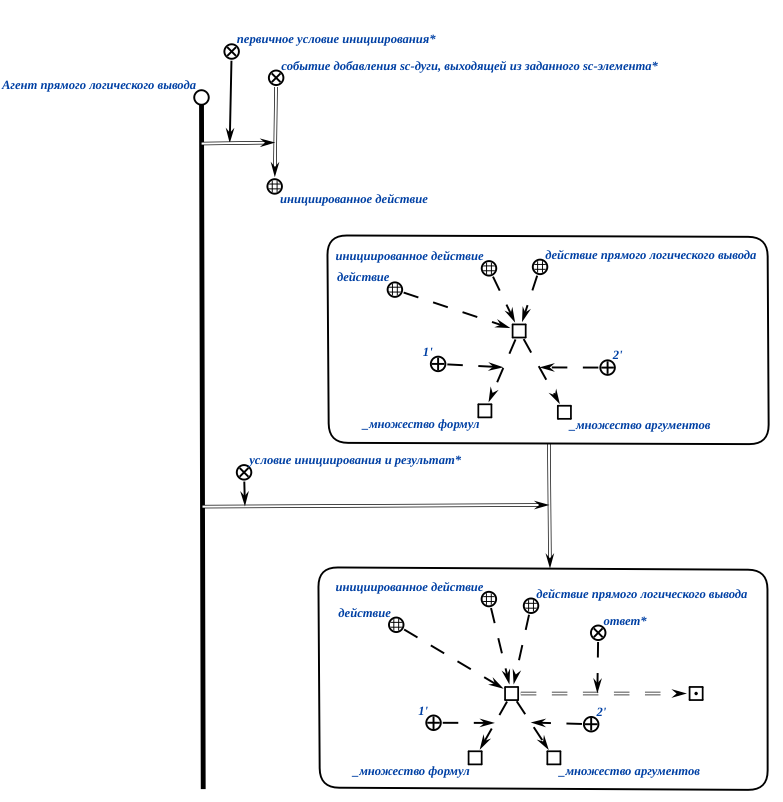
\includegraphics[width=0.9\linewidth, height=8cm]{figures/sc-agents/direct_inference_agent.png}
\end{figure}
\end{frame}

<<<<<<< Updated upstream
\begin{frame}{\Large Абстрактный sc-агент обратного логического вывода}
\vspace{8mm}
  Абстрактный sc-агент обратного логического вывода проверяет гипотезы. Некоторые гипотезы могут быть опровергнуты, однако извлекая причины того, почему гипотеза опровергнута, можно изменить посылку гипотезы так, чтобы создать новую гипотезу, которая впоследствии может стать полезной теоремой. Данный sc-агент активируется при появлении в sc-памяти инициированного действия, принадлежащего классу действие обратного логического вывода. После проверки sc-агентом условия инициирования выполняется процесс обратного логического вывода, который схож с процессом прямого логического вывода за исключением того, что поиск правил основывается не на посылках формул, а на их следствиях. Ответом данного агента будет также дерево вывода, которое показывает, с использованием каких правил можно доказать или опровергнуть выдвинутую гипотезу. 
\end{frame}

\begin{frame}{\\Принципы синхронизации деятельности sc-агентов}
=======
\begin{frame}{Абстрактный sc-агент обратного логического вывода}
\topline
\vspace{30
}
 \\

  Абстрактный sc-агент обратного логического вывода проверяет гипотезы. Некоторые гипотезы могут быть опровергнуты, однако извлекая причины того, почему гипотеза опровергнута, можно изменить посылку гипотезы так, чтобы создать новую гипотезу, которая впоследствии может стать полезной теоремой. Данный sc-агент активируется при появлении в sc-памяти инициированного действия, принадлежащего классу действие обратного логического вывода. После проверки sc-агентом условия инициирования выполняется процесс обратного логического вывода, который схож с процессом прямого логического вывода за исключением того, что поиск правил основывается не на посылках формул, а на их следствиях. Ответом данного агента будет также дерево вывода, которое показывает, с использованием каких правил можно доказать или опровергнуть выдвинутую гипотезу. 
\end{frame}

\begin{frame}{Принципы синхронизации деятельности sc-агентов}
\topline
\vspace{30}
 \\
 
>>>>>>> Stashed changes
        Одной из важных особенностей многоагентного подхода к решению задач является возможность параллельного решения различных задач, что в свою очередь, предполагает параллельность выполнения соответствующих информационных процессов.
        Понятия \textit{действие в sc-памяти}, и \textit{процесс в sc-памяти} (\textit{информационный процесс}, выполняемый агентом в семантической памяти), являются синонимичными, поскольку все процессы, протекающие в sc-памяти, являются осознанными и выполняются каким-либо \textit{sc-агентами}. Тем не менее, когда идет речь о синхронизации выполнения каких-либо преобразований в памяти компьютерной системы, в литературе принято использовать именно термины ``процесс'', ``взаимодействие процессов''
\end{frame}

<<<<<<< Updated upstream
\begin{frame}{Блокировки}
=======
\begin{frame}{\\Блокировки}
\topline
\vspace{30}
 \\

>>>>>>> Stashed changes
Для синхронизации выполнения \textit{процессов в sc-памяти} предлагается использовать механизм блокировок, построенный на основе существующих алгоритмов синхронизации информационных процессов в традиционных системах. В качестве возможного направления развития данного подхода можно указать набирающие популярность идеи lock-free алгоритмов.

Отношение \textbf{\textit{блокировка*}} связывает знаки \textit{действий в sc-памяти} со знаками \textit{структур} (ситуативных), которые содержат элементы, заблокированные на время выполнения данного действия или на какую-то часть этого периода. Каждая такая \textit{структура} принадлежит какому-либо из \textit{типов блокировки}.

Первым компонентом связок отношения \textbf{\textit{блокировка*}} является знак \textit{действия в sc-памяти}, вторым --- знак заблокированной \textit{структуры}.
\end{frame}

\begin{frame}{\\Блокировка}
<<<<<<< Updated upstream
=======
\topline
>>>>>>> Stashed changes
  \scnheader{блокировка*}
\scniselement{бинарное отношение}
\scnheader{тип блокировки}
\scnhaselement{полная блокировка}
\scnhaselement{блокировка на любое изменение}
\scnhaselement{блокировка на удаление}  
\end{frame}

<<<<<<< Updated upstream
\begin{frame}{}
    \caption{SCg-текст. Пример использования блокировок}
	\includegraphics[width=0.9\linewidth, height=8cm]{scn-slides/figures/plan_lock_1.png}
\end{frame}

\begin{frame}{ Полная блокировка}
\vspace{12}
=======
\newpage
\begin{figure}
    \centering
    \caption{Пример использования блокировок}
	\includegraphics[width=0.9\linewidth, height=7cm]{scn-slides/figures/plan_lock_1.png}
\end{figure}
    


\begin{frame}{\\Полная блокировка}
\topline
\vspace{30}
 \\

>>>>>>> Stashed changes
   Каждая \textit{структура}, принадлежащая множеству \textbf{\textit{полная блокировка}} содержит \textit{sc-элементы}, просмотр и изменение которых запрещены всем \textit{sc-агентам}, кроме собственно \textit{sc-агента}, выполняющего соответствующее данной структуре \textit{действие в sc-памяти}, связанное с ней отношением \textit{блокировка*}.
\\Для того, чтобы исключить возможность реализации \textit{sc-агентов}, которые могут внести изменения в конструкции, описывающие блокировки других \textit{sc-агентов}, все элементы этих конструкций, в том числе, сам знак \textit{структуры}, содержащей заблокированные \textit{sc-элементы} (принадлежащей как множеству \textbf{\textit{полная блокировка}}, так и любому другому \textit{типу блокировки}) и связки отношения \textit{блокировка*}, связывающие эту \textit{структуру} и конкретное \textit{действие в sc-памяти}, добавляются в \textbf{\textit{полную блокировку}}, соответствующую данному \textit{действию в sc-памяти}. Таким образом, каждой \textbf{\textit{полной блокировке}} соответствует петля принадлежности, связывающая ее знак с самим собой. 
\end{frame}

<<<<<<< Updated upstream
\begin{frame}{Блокировка на любое изменение}
  Каждая \textit{структура}, принадлежащая множеству \textbf{\textit{блокировка на любое изменение}} содержит \textit{sc-элементы}, изменение (физическое удаление, добавление инцидентных \textit{sc-коннекторов}, физическое удаление самих \textit{\mbox{sc-элементов}}, изменение содержимого в случае файла) которых запрещено всем \textit{sc-агентам}, кроме собственно \textit{sc-агента}, выполняющего соответствующее данной структуре \textit{действие в sc-памяти}, связанное с ней отношением \textit{блокировка*}. Однако не запрещен просмотр (чтение) этих \textit{sc-элементов} любым \textit{sc-агентом}.  
\end{frame}

\begin{frame}{Блокировка на удаление}
=======
\begin{frame}{\\Блокировка на любое изменение}
\topline
\vspace{15}
 \\

  Каждая \textit{структура}, принадлежащая множеству \textbf{\textit{блокировка на любое изменение}} содержит \textit{sc-элементы}, изменение (физическое удаление, добавление инцидентных \textit{sc-коннекторов}, физическое удаление самих \textit{\mbox{sc-элементов}}, изменение содержимого в случае файла) которых запрещено всем \textit{sc-агентам}, кроме собственно \textit{sc-агента}, выполняющего соответствующее данной структуре \textit{действие в sc-памяти}, связанное с ней отношением \textit{блокировка*}. Однако не запрещен просмотр (чтение) этих \textit{sc-элементов} любым \textit{sc-агентом}.  
\end{frame}

\begin{frame}{\\Блокировка на удаление}
\topline
\vspace{15}
 \\

>>>>>>> Stashed changes
  Каждая \textit{структура}, принадлежащая множеству \textbf{\textit{блокировка на удаление}} содержит \textit{sc-элементы}, удаление которых запрещено всем \textit{sc-агентам}, кроме собственно \textit{sc-агента}, выполняющего соответствующее данной структуре \textit{действие в sc-памяти}, связанное с ней отношением \textit{блокировка*}. Однако не запрещен просмотр (чтение) этих \textit{sc-элементов} любым \textit{sc-агентом}, добавление инцидентных sc-коннекторов.  
\end{frame}
    
    
\begin{frame}{Принципы работы с блокировками}
<<<<<<< Updated upstream
=======
\topline
\vspace{30}
 \\

>>>>>>> Stashed changes
\begin{textitemize}
	\item в каждый момент времени одному \textit{процессу в sc-памяти} может соответствовать только одна блокировка каждого типа;
	\item в каждый момент времени одному \textit{процессу в sc-памяти} может соответствовать только одна блокировка, установленная на некоторый конкретный sc-элемент;
	\item при завершении выполнения любого \textit{процесса в sc-памяти} все установленные им блокировки автоматически снимаются;
	\item для повышения эффективности работы системы в целом каждый процесс должен в каждый момент времени блокировать минимально необходимое множество sc-элементов, снимая блокировку с каждого sc-элемента сразу же, как это становится возможным (безопасным);    
    \end{textitemize}
    \end{frame}
<<<<<<< Updated upstream
=======
    \begin{frame}{}
    \vspace{30}
     \\

>>>>>>> Stashed changes
        \begin{textitemize}
        \item В случае когда в рамках \textit{процесса в sc-памяти} явно выделяются более частные подпроцессы (при помощи отношений \textit{темпоральная часть*, поддействие*, декомпозиция действия*} и так далее), то каждый такой подпроцесс с точки зрения синхронизации выполнения рассматривается как самостоятельный процесс, которому в соответствие могут быть поставлены все необходимые блокировки.
	    \item все дочерние процессы в sc-памяти имеют доступ к блокировкам родительского процесса так же, как если бы это были блокировки соответствующие каждому из таких дочерних процессов;
		\item в свою очередь, родительский процесс не имеет какого-либо привилегированного доступа к sc-элементам, заблокированным дочерними процессами, и работает с ними так же, как любой другой процесс в sc-памяти. Исключение составляют sc-элементы, обозначающие сами дочерние процессы, поскольку родительский процесс должен иметь возможность управления дочерним, например, приостановки или прекращения их выполнения;
<<<<<<< Updated upstream
		\item все дочерние процессы по отношению друг к другу работают так же, как и по отношению к любым другим процессам;
		\newpage 
        \item в случае, когда родительский процесс приостанавливает выполнение (становится \textit{отложенным действием}), \uline{все} его дочерние процессы также приостанавливают выполнение. В свою очередь, приостановка одного из дочерних процессов в общем случае не инициирует явно остановку всего родительского процесса и соответственно других дочерних.
		\end{textitemize}
\begin{frame}{\large Принципы работы с полными блокировками}
    \vspace{18}
=======
  \end{textitemize}
  \end{frame}
  \begin{frame}{}
      \begin{textitemize}
        \item все дочерние процессы по отношению друг к другу работают так же, как и по отношению к любым другим процессам; 
        \item в случае, когда родительский процесс приостанавливает выполнение (становится \textit{отложенным действием}), \uline{все} его дочерние процессы также приостанавливают выполнение. В свою очередь, приостановка одного из дочерних процессов в общем случае не инициирует явно остановку всего родительского процесса и соответственно других дочерних.
		\end{textitemize}
\end{frame}

\begin{frame}{\\Принципы работы с полными блокировками}
\topline
    \vspace{30}
     \\

>>>>>>> Stashed changes
    \begin{textitemize}
	\item если sc-элемент, инцидентный некоторому sc-коннектору, попадает в какую-либо полную блокировку, то сам этот sc-коннектор по умолчанию также считается заблокированным этой же блокировкой. Обратное в общем случае неверно, так как часть sc-коннекторов, инцидентных некоторому sc-элементу, может быть полностью заблокирована, при этом сам этот элемент заблокирован не будет. Такая ситуация типична, например, для sc-узлов, обозначающих классы понятий;
	\item каждый процесс в sc-памяти может свободно изменять или удалять любые sc-элементы, попадающие в полную блокировку, соответствующую этому процессу.
\end{textitemize}
Следует понимать, что все процессы, кроме установившего полную блокировку, не имеют доступа к заблокированным элементам(не вызывают конфликты). С другой стороны частое использование таких блокировок может привести к тому, что система не сможет использовать все имеющиеся знания.
\end{frame}

<<<<<<< Updated upstream
\begin{frame}{\large Принципы работы с блокировками на любое изменение или удаление}
\vspace{18}
=======
\begin{frame}{Принципы работы с блокировками на любое изменение или удаление}
\topline
\vspace{30}
 \\

>>>>>>> Stashed changes
    \begin{textitemize}
	\item на один и тот же sc-элемент в один момент времени может быть установлена только одна блокировка одного типа, но разные процессы могут одновременно установить на один и тот же элемент блокировки двух разных типов. Это касается случая, когда первый процесс установил на некоторый sc-элемент блокировку на удаление, а второй процесс затем устанавливает блокировку на любое изменение. В других случаях возникает конфликт блокировок;
	\item установка блокировки любого типа также считается изменением. Если на некоторый \mbox{sc-элемент} была установлена блокировка на любое изменение, то другой процесс не сможет установить на этот же sc-элемент блокировку, пока первый процесс не снимет свою;
	\item если блокировка на удаление устанавливается на некоторый sc-коннектор, то по умолчанию та же блокировка устанавливается на инцидентные этому sc-коннектору sc-элементы, поскольку удаление этих элементов приведет к удалению этого коннектора.
\end{textitemize}
\end{frame}

<<<<<<< Updated upstream
\begin{frame}{\large Классификация процессов в sc-памяти с точки зрения синхронизации их выполнения}
\vspace{15}
\begin{textitemize}
    \item{действие поиска sc-элементов}
	\item{действие генерации sc-элементов}
	\item{действие удаления sc-элементов}
	\item{действие установки блокировки некоторого типа на некоторый sc-элемент}
	\item{действие снятия блокировки с некоторого sc-элемента}
 \end{textitemize}
 В некоторых случаях для обеспечения синхронизации необходимо объединять несколько элементарных действий над sc-памятью в одно неделимое действие с гарантией того, что ни один сторонний процесс не сможет прочитать или изменить участвующие в этом действии sc-элементы до завершения действия. При этом, пытающийся получить доступ к таким элементам процесс ожидает завершения действия, после чего может выполнять с ними любые действия согласно принципам синхронизации.
\end{frame}

В случае выполнения \textit{действия поиска sc-элементов} все найденные и сохраненные в рамках какого-либо процесса sc-элементы попадают в соответствующую данному процессу \textit{блокировку на любое изменение}. Таким образом, гарантируется целостность фрагмента базы знаний, с которым работает некоторый процесс в sc-памяти. При этом поиск и автоматическая установка такой блокировки должны быть реализованы как \textit{транзакция в sc-памяти}.
	
Такой подход также позволяет избежать ситуации, когда один процесс заблокировал некоторый sc-элемент на любое изменение, а второй процесс пытается сгенерировать или удалить \textit{sc-коннектор}, инцидентный данному \textit{sc-элементу}. В таком случае второй процесс должен будет предварительно найти и заблокировать указанный \textit{sc-элемент} на любое изменение, что вызовет конфликт блокировок (\textit{взаимоблокировку*}).

В случае генерации любого sc-элемента в рамках некоторого процесса он автоматически попадает в полную блокировку, соответствующую данному процессу. При этом генерация и автоматическая установка такой блокировки должны быть реализованы как \textit{транзакция в sc-памяти}. При необходимости сгенерированные элементы могут быть удалены (их временное существование никак не отразится на деятельности других процессов) или разблокированы в случае, когда сгенерирована информация, которая может иметь некоторую ценность в дальнейшем.

В случае если какой-либо процесс пытается установить блокировку любого типа на какой-либо sc-элемент, уже заблокированный каким-либо другим процессом, то, с одной стороны, блокировка не может быть установлена, пока другой процесс не разблокирует указанный sc-элемент; с другой стороны, для того чтобы обеспечить возможность поиска и устранения \textit{взаимоблокировок}, необходимо явно указывать тот факт, что какой-либо процесс хочет получить доступ к какому-либо заблокированному другим процессом sc-элементу. Для того чтобы иметь возможность указать, какие процессы пытаются заблокировать уже заблокированный \textit{sc-элемент}, предлагается наряду с отношением \textit{блокировка*} использовать отношение \textit{планируемая блокировка*}, полностью аналогичное отношению \textit{блокировка*}.
	
Описанный механизм регулирует также и процессы поиска, поскольку поиск и сохранение некоторого sc-элемента предполагает установку \textit{блокировки на любое изменение}. Кроме того, следует учитывать, что на один sc-элемент \textit{блокировка на любое изменение} может быть установлена после \textit{блокировки на удаление}, соответствующей другому процессу. В этом случае использовать отношение \textit{планируемые блокировки*} нет необходимости.
	
Действие проверки наличия на некотором sc-элементе блокировки и в зависимости от результата проверки, установки блокировки или планируемой блокировки (с указанием приоритета при необходимости) должно быть реализовано как транзакция.

\begin{frame}{Связь с базовым языком программирования для обработки баз
знаний}
\vspace{15}
=======
\begin{frame}{\\Процесс в sc-памяти}
\topline
\vspace{30}
 \\
\begin{SCn}
\scnheader{процесс в sc-памяти}
\scnrelfrom{разбиение}{Классификация процессов в sc-памяти с точки зрения синхронизации их выполнения}
\begin{scnindent}
\begin{scneqtoset}
	\scnitem{действие поиска sc-элементов}
	\scnitem{действие генерации sc-элементов}
	\scnitem{действие удаления sc-элементов}
	\scnitem{действие установки блокировки некоторого типа на некоторый sc-элемент}
	\scnitem{действие снятия блокировки с некоторого sc-элемента}
\end{scneqtoset}
\end{scnindent}
\end{SCn}
\end{frame}

\begin{frame}{}
В некоторых случаях для обеспечения синхронизации необходимо объединять несколько элементарных действий над sc-памятью в одно неделимое действие с гарантией того, что ни один сторонний процесс не сможет прочитать или изменить участвующие в этом действии sc-элементы до завершения действия. При этом, пытающийся получить доступ к таким элементам процесс ожидает завершения действия, после чего может выполнять с ними любые действия согласно принципам синхронизации.

В случае выполнения \textit{действия поиска sc-элементов} все найденные и сохраненные в рамках какого-либо процесса sc-элементы попадают в соответствующую данному процессу \textit{блокировку на любое изменение}. Таким образом, гарантируется целостность фрагмента базы знаний, с которым работает некоторый процесс в sc-памяти. При этом поиск и автоматическая установка такой блокировки должны быть реализованы как \textit{транзакция в sc-памяти}.
	
\end{frame}

\begin{frame}{}
Такой подход также позволяет избежать ситуации, когда один процесс заблокировал некоторый sc-элемент на любое изменение, а второй процесс пытается сгенерировать или удалить \textit{sc-коннектор}, инцидентный данному \textit{sc-элементу}. В таком случае второй процесс должен будет предварительно найти и заблокировать указанный \textit{sc-элемент} на любое изменение, что вызовет конфликт блокировок (\textit{взаимоблокировку*}).

В случае генерации любого sc-элемента в рамках некоторого процесса он автоматически попадает в полную блокировку, соответствующую данному процессу. При этом генерация и автоматическая установка такой блокировки должны быть реализованы как \textit{транзакция в sc-памяти}. При необходимости сгенерированные элементы могут быть удалены (их временное существование никак не отразится на деятельности других процессов) или разблокированы в случае, когда сгенерирована информация, которая может иметь некоторую ценность в дальнейшем.
\end{frame}

\begin{frame}{}
В случае если какой-либо процесс пытается установить блокировку любого типа на какой-либо sc-элемент, уже заблокированный каким-либо другим процессом, то, с одной стороны, блокировка не может быть установлена, пока другой процесс не разблокирует указанный sc-элемент; с другой стороны, для того чтобы обеспечить возможность поиска и устранения \textit{взаимоблокировок}, необходимо явно указывать тот факт, что какой-либо процесс хочет получить доступ к какому-либо заблокированному другим процессом sc-элементу. Для того чтобы иметь возможность указать, какие процессы пытаются заблокировать уже заблокированный \textit{sc-элемент}, предлагается наряду с отношением \textit{блокировка*} использовать отношение \textit{планируемая блокировка*}, полностью аналогичное отношению \textit{блокировка*}.
\end{frame}

\begin{frame}{}
Описанный механизм регулирует также и процессы поиска, поскольку поиск и сохранение некоторого sc-элемента предполагает установку \textit{блокировки на любое изменение}. Кроме того, следует учитывать, что на один sc-элемент \textit{блокировка на любое изменение} может быть установлена после \textit{блокировки на удаление}, соответствующей другому процессу. В этом случае использовать отношение \textit{планируемые блокировки*} нет необходимости.
	
Действие проверки наличия на некотором sc-элементе блокировки и в зависимости от результата проверки, установки блокировки или планируемой блокировки (с указанием приоритета при необходимости) должно быть реализовано как транзакция.
\end{frame}

\begin{frame}{Связь с базовым языком программирования для обработки баз знаний}
\topline
\vspace{30}
 \\

>>>>>>> Stashed changes
    Выделение Базового языка программирования для ostis-систем позволяет обеспечить четкое разделение уровня методов и соответственно, навыков ostis-системы, которые могут быть полностью описаны на уровне базы знаний и более низкоуровневых навыков, обеспечивающих интерпретацию указанных навыков более высокого уровня. Другими словами, выделение такого языка позволяет обеспечить \uline{платформенную независимость} ostis-систем, как в случае программной реализации \textit{ostis-платформы}, так и в случае \textit{ассоциативного семантического компьютера}.
    \par В качестве базового языка для описания программ обработки текстов \textit{SC-кода} предлагается \textit{Язык SCP}. \textbf{\textit{Язык SCP}} -- это графовый язык процедурного программирования, предназначенный для эффективной обработки \textit{sc-текстов}. \textit{Язык SCP} является языком параллельного асинхронного программирования.
\end{frame}

<<<<<<< Updated upstream
Языком представления данных для текстов Языка SCP (scp-программ) является SC-код и, соответственно, любые варианты его внешнего представления. Язык SCP сам построен на основе SC-кода, вследствие чего scp-программы сами по себе могут входить в состав обрабатываемых данных для scp-программ, в том числе по отношению к самим себе. Таким образом, Язык SCP предоставляет возможность построения реконфигурируемых программ. Однако для обеспечения возможности реконфигурирования программы непосредственно в процессе ее интерпретации необходимо на уровне интерпретатора Языка SCP (Aбстрактной scp-машины) обеспечить уникальность каждой исполняемой копии исходной программы. Такую исполняемую копию, сгенерированную на основе scp-программы, будем называть scp-процессом. Включение знака некоторого действия в sc-памяти во множество scp-процессов гарантирует тот факт, что в декомпозиции данного действия будут присутствовать только знаки элементарных действий (scp-операторов), которые может интерпретировать реализация Aбстрактной scp-машины (интерпретатора scp-программ).

\begin{frame}{Особенности и достоинства Базовой модели обработки sc-текстов}
\vspace{15}
=======
\begin{frame}{}
\vspace{30}
 \\

Языком представления данных для текстов Языка SCP (scp-программ) является SC-код и, соответственно, любые варианты его внешнего представления. Язык SCP сам построен на основе SC-кода, вследствие чего scp-программы сами по себе могут входить в состав обрабатываемых данных для scp-программ, в том числе по отношению к самим себе. Таким образом, Язык SCP предоставляет возможность построения реконфигурируемых программ. Однако для обеспечения возможности реконфигурирования программы непосредственно в процессе ее интерпретации необходимо на уровне интерпретатора Языка SCP (Aбстрактной scp-машины) обеспечить уникальность каждой исполняемой копии исходной программы. Такую исполняемую копию, сгенерированную на основе scp-программы, будем называть scp-процессом. Включение знака некоторого действия в sc-памяти во множество scp-процессов гарантирует тот факт, что в декомпозиции данного действия будут присутствовать только знаки элементарных действий (scp-операторов), которые может интерпретировать реализация Aбстрактной scp-машины (интерпретатора scp-программ).
\end{frame}

\begin{frame}{Особенности и достоинства Базовой модели обработки sc-текстов}
\topline
\vspace{30}
 \\

>>>>>>> Stashed changes
\begin{textitemize}
    \item Тексты программ \textit{Языка SCP} записываются при помощи тех же унифицированных семантических сетей, что и обрабатываемая информация, таким образом, можно сказать, что \textit{Синтаксис Языка SCP} на базовом уровне совпадает с \textit{Синтаксисом SC-кода}.
    \item Подход к интерпретации \textit{scp-программ} предполагает создание при каждом вызове \textit{scp-программы} уникального \textit{scp-процесса}.
    \item Одновременно в общей памяти могут выполняться несколько независимых \textit{sc-агентов}, при этом разные копии \textit{sc-агентов} могут выполняться на разных серверах, за счет распределенной реализации \textit{ostis-платформы}. Более того, \textit{Язык SCP} позволяет осуществлять параллельные асинхронные вызовы подпрограмм с последующей синхронизацией, и даже параллельно	выполнять операторы в рамках одной \textit{scp-программы}.
    \end{textitemize}
\end{frame}
<<<<<<< Updated upstream
=======

\begin{frame}{}
\vspace{30}
 \\

>>>>>>> Stashed changes
\begin{textitemize}
    \item Перенос \textit{sc-агента} из одной системы в другую заключается в простом переносе фрагмента \textit{базы знаний}, без каких-либо дополнительных операций, зависящих от \textit{ostis-платформы}.
	\item Тот факт, что спецификации \textit{sc-агентов} и их программы могут быть записаны на том же языке, что и обрабатываемые знания, существенно сокращает перечень специализированных средств, предназначенных для проектирования машин обработки знаний, и упрощает их разработку за счет использования более универсальных компонентов.
	\item Тот факт, что для интерпретации \textit{scp-программы} создается соответствующий ей уникальный \textit{\mbox{scp-процесс}}, позволяет по возможности оптимизировать план выполнения перед его реализацией и даже непосредственно в процессе выполнения без потенциальной опасности испортить общий универсальный алгоритм всей программы. Более того, такой подход к проектированию и интерпретации программ позволяет говорить о возможности создания самореконфигурируемых программ.
\end{textitemize}
<<<<<<< Updated upstream

\newpage
Каждая \textbf{\textit{scp-программа}} представляет собой обобщенную \textit{sc-структуру}, описывающую один из вариантов декомпозиции действий некоторого класса, выполняемых в sc-памяти. Знак \textit{sc-переменной}, соответствующей конкретному декомпозируемому действию является в рамках \textbf{\textit{scp-программы}} \textit{ключевым sc-элементом\scnrolesign}. Также явно указывается принадлежность данного знака множеству \textit{scp-процессов}.
	
Принадлежность некоторого действия множеству \textit{scp-процессов} гарантирует тот факт, что в декомпозиции данного действия будут присутствовать только знаки элементарных действий (\textit{scp-операторов}), которые может интерпретировать реализация \textit{Абстрактной scp-машины}.

=======
\end{frame}

\begin{frame}{}
Каждая \textbf{\textit{scp-программа}} представляет собой обобщенную \textit{sc-структуру}, описывающую один из вариантов декомпозиции действий некоторого класса, выполняемых в sc-памяти. Знак \textit{sc-переменной}, соответствующей конкретному декомпозируемому действию является в рамках \textbf{\textit{scp-программы}} \textit{ключевым sc-элементом\scnrolesign}. Также явно указывается принадлежность данного знака множеству \textit{scp-процессов}.
	
Принадлежность некоторого действия множеству \textit{scp-процессов} гарантирует тот факт, что в декомпозиции данного действия будут присутствовать только знаки элементарных действий (\textit{scp-операторов}), которые может интерпретировать реализация \textit{Абстрактной scp-машины}.
\end{frame}

\begin{frame}{}
>>>>>>> Stashed changes
Таким образом, каждая \textbf{\textit{scp-программа}} описывает в обобщенном виде декомпозицию некоторого \textit{\mbox{scp-процесса}} на взаимосвязанные \textit{scp-операторы}, с указанием, при их наличии, аргументов для данного \textit{scp-процесса}.

По сути каждая \textbf{\textit{scp-программа}} представляет собой описание последовательности элементарных операций, которые необходимо выполнить над семантической сетью, чтобы выполнить более сложное действие некоторого класса.
На рисунке приведен пример простой \textit{scp-программы}. В примере показана \textit{scp-программа}, состоящая из трех \textit{scp-операторов}. Данная программа проверяет, содержится ли в заданном множестве (первый параметр) заданный элемент (второй параметр), и, если нет, то добавляет его в это множество.
<<<<<<< Updated upstream
=======
\end{frame}
>>>>>>> Stashed changes

\begin{frame}{}
\begin{figure}[H]
    \caption{SCg-текст. Пример scp-программы}
	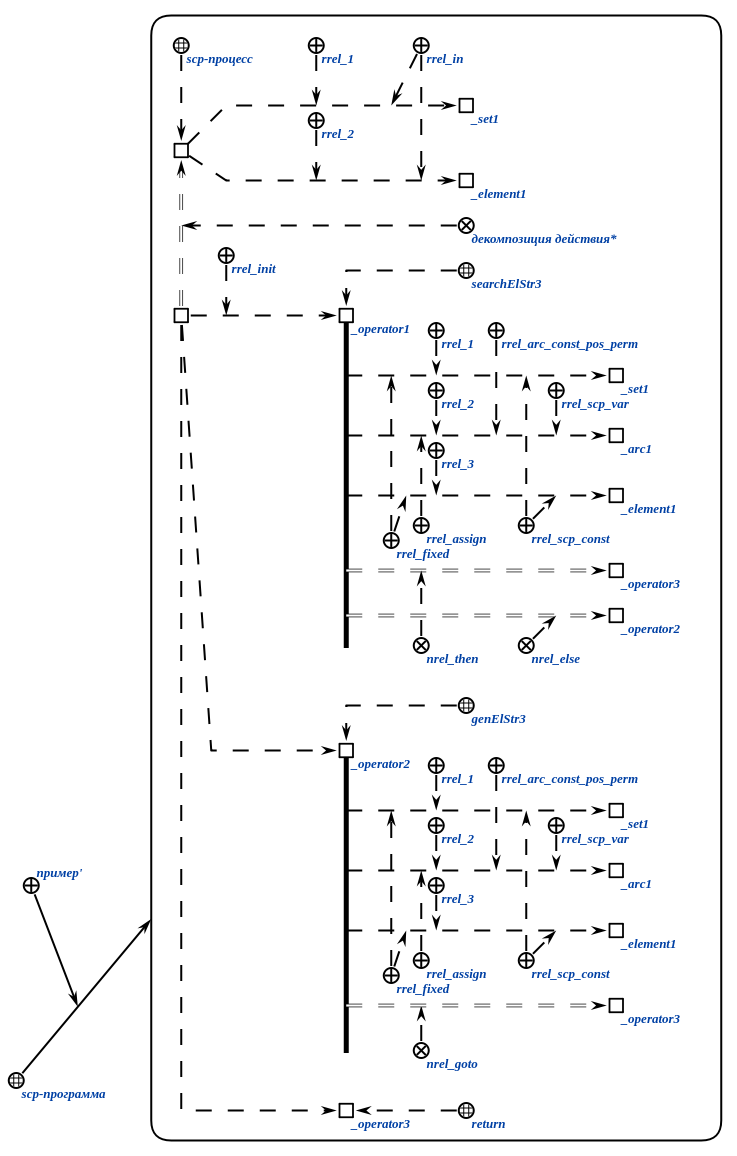
\includegraphics[width=0.9\linewidth, height=8cm]{figures/sc-agents/program_example.png}
\end{figure}
\end{frame}

<<<<<<< Updated upstream
\textbf{\textit{Агентные scp-программы}} представляют собой частный случай \textit{scp-программ} вообще, однако заслуживают отдельного рассмотрения, поскольку используются наиболее часто. \textit{scp-программы} данного класса представляют собой реализации программ агентов обработки знаний, и имеют жестко фиксированный набор параметров. Каждая такая программа имеет ровно два \textit{in-параметра\scnrolesign}. Значение первого параметра является знаком бинарной ориентированной пары, являющейся вторым компонентом связки отношения \textit{первичное условие инициирования*} для абстрактного \textit{sc-агента}, в множество \textit{программ sc-агента*} которого входит рассматриваемая \textbf{\textit{агентная scp-программа}}, и, по сути, описывает класс событий, на которые реагирует указанный sc-агент.
	
Значением второго параметра является \textit{sc-элемент}, с которым непосредственно связано событие, в результате возникновения которого был инициирован соответствующий \textit{sc-агент}, то есть, например, сгенерированная либо удаляемая \textit{sc-дуга} или \textit{sc-ребро}.

\begin{frame}{\large Принципы реализации абстрактных sc-агентов, реализуемых на Языке SCP}
\vspace{15}
=======
\begin{frame}{}
\vspace{40}
 \\

\textbf{\textit{Агентные scp-программы}} представляют собой частный случай \textit{scp-программ} вообще, однако заслуживают отдельного рассмотрения, поскольку используются наиболее часто. \textit{scp-программы} данного класса представляют собой реализации программ агентов обработки знаний, и имеют жестко фиксированный набор параметров. Каждая такая программа имеет ровно два \textit{in-параметра\scnrolesign}. Значение первого параметра является знаком бинарной ориентированной пары, являющейся вторым компонентом связки отношения \textit{первичное условие инициирования*} для абстрактного \textit{sc-агента}, в множество \textit{программ sc-агента*} которого входит рассматриваемая \textbf{\textit{агентная scp-программа}}, и, по сути, описывает класс событий, на которые реагирует указанный sc-агент.
	
Значением второго параметра является \textit{sc-элемент}, с которым непосредственно связано событие, в результате возникновения которого был инициирован соответствующий \textit{sc-агент}, то есть, например, сгенерированная либо удаляемая \textit{sc-дуга} или \textit{sc-ребро}.
\end{frame}

\begin{frame}{Принципы реализации абстрактных sc-агентов, реализуемых на Языке SCP}
\topline
\vspace{30}
 \\

>>>>>>> Stashed changes
    \begin{textitemize}
    \item общие принципы организации взаимодействия \textit{sc-агентов} и пользователей \textit{ostis-системы} через общую \textit{sc-память};
\item в результате появления в sc-памяти некоторой конструкции, удовлетворяющей условию инициирования какого-либо \textit{абстрактного sc-агента}, реализованного при помощи \textit{Языка SCP}, в \textit{sc-памяти} генерируется и инициируется \textit{scp-процесс}. В качестве шаблона для генерации используется \textit{агентная scp-программа}, указанная во множестве программ соответствующего \textit{абстрактного sc-агента};
\item каждый такой \textit{scp-процесс}, соответствующий некоторой \textit{агентной scp-программе}, может быть связан с набором структур, описывающих блокировки различных типов. Таким образом, синхронизация взаимодействия параллельно выполняемых \textit{scp-процесcов} осуществляется так же, как и в случае любых других \textit{действий в sc-памяти};
\end{textitemize}
\end{frame}

<<<<<<< Updated upstream
\begin{textitemize}
    \item В рамках \textit{scp-процесса} могут создаваться дочерние \textit{scp-процессы}, однако синхронизация между ними при необходимости осуществляется посредством введения дополнительных внутренних блокировок. Таким образом, каждый \textit{scp-процесс} с точки зрения \textit{процессов в sc-памяти} является атомарным и законченным актом деятельности некоторого \textit{sc-агента};
\item во избежание нежелательных изменений в самом теле \textit{scp-процесса}, вся конструкция, сгенерированная на основе некоторой \textit{scp-программы} (весь текст \textit{scp-процесса}), должна быть добавлена в \textit{полную блокировку}, соответствующую данному \textit{scp-процессу};
\item все конструкции, сгенерированные в процессе выполнения
\textit{scp-процесса}, автоматически попадают в \textit{полную 	блокировку}, соответствующую данному \textit{scp-процессу}. Дополнительно следует отметить, что знак самой этой структуры и вся метаинформация о ней также включаются в эту структуру;
\item при необходимости можно вручную разблокировать или заблокировать некоторую конструкцию каким-либо типом блокировки, используя соответствующие \textit{scp-операторы} класса \textit{scp-оператор управления блокировками};
\item после завершения выполнения некоторого \textit{scp-процесса} его текст как правило, удаляется из \textit{\mbox{sc-памяти}}, а все заблокированные конструкции освобождаются (разрушаются знаки структур, обозначавших блокировки);
\item несмотря на то, что каждый \textit{scp-оператор} представляет собой атомарное \textit{действие в sc-памяти}, дополнительные блокировки, соответствующие одному оператору не вводятся, чтобы избежать громоздкости и избытка дополнительных системных конструкций, создаваемых при выполнении некоторого \textit{scp-процесса}. Вместо этого используются блокировки, общие для всего \textit{scp-процесса}. Таким образом, агенты \textit{Абстрактной scp-машины} при интерпретации \textit{scp-операторов} работают только с учетом блокировок, общих для всего интерпретируемого \textit{scp-процесса};
\item как правило, частный \textit{класс действий}, соответствующий конкретной \textit{scp-программе} явно не вводится, а используется более общий класс \textit{scp-процесс}, за исключением тех случаев, когда введение специального \textit{класса действий} необходимо по каким-либо другим соображениям.
\end{textitemize}
=======
\begin{frame}{}
\begin{textitemize}
    \item В рамках \textit{scp-процесса} могут создаваться дочерние \textit{scp-процессы}, однако синхронизация между ними при необходимости осуществляется посредством введения дополнительных внутренних блокировок. Таким образом, каждый \textit{scp-процесс} с точки зрения \textit{процессов в sc-памяти} является атомарным и законченным актом деятельности некоторого \textit{sc-агента};
    \item во избежание нежелательных изменений в самом теле \textit{scp-процесса}, вся конструкция, сгенерированная на основе некоторой \textit{scp-программы} (весь текст \textit{scp-процесса}), должна быть добавлена в \textit{полную блокировку}, соответствующую данному \textit{scp-процессу};
\end{textitemize}
\end{frame}

\begin{frame}{}
\begin{textitemize}
\item все конструкции, сгенерированные в процессе выполнения \textit{scp-процесса}, автоматически попадают в \textit{полную 	блокировку}, соответствующую данному \textit{scp-процессу}. Дополнительно следует отметить, что знак самой этой структуры и вся метаинформация о ней также включаются в эту структуру;
\item при необходимости можно вручную разблокировать или заблокировать некоторую конструкцию каким-либо типом блокировки, используя соответствующие \textit{scp-операторы} класса \textit{scp-оператор управления блокировками};
\item после завершения выполнения некоторого \textit{scp-процесса} его текст как правило, удаляется из \textit{\mbox{sc-памяти}}, а все заблокированные конструкции освобождаются (разрушаются знаки структур, обозначавших блокировки);
\end{textitemize}
\end{frame}

\begin{frame}{}
\begin{textitemize}
\item несмотря на то, что каждый \textit{scp-оператор} представляет собой атомарное \textit{действие в sc-памяти}, дополнительные блокировки, соответствующие одному оператору не вводятся, чтобы избежать громоздкости и избытка дополнительных системных конструкций, создаваемых при выполнении некоторого \textit{scp-процесса}. Вместо этого используются блокировки, общие для всего \textit{scp-процесса}. Таким образом, агенты \textit{Абстрактной scp-машины} при интерпретации \textit{scp-операторов} работают только с учетом блокировок, общих для всего интерпретируемого \textit{scp-процесса};
\item как правило, частный \textit{класс действий}, соответствующий конкретной \textit{scp-программе} явно не вводится, а используется более общий класс \textit{scp-процесс}, за исключением тех случаев, когда введение специального \textit{класса действий} необходимо по каким-либо другим соображениям.
\end{textitemize}
\end{frame}
>>>>>>> Stashed changes
